\documentclass[10pt,journal,onecolumn]{IEEEtran}

\usepackage{amsmath,amssymb}
\usepackage{booktabs}
\usepackage{graphicx}
\usepackage{multirow}
\usepackage{xcolor}
\usepackage[hidelinks]{hyperref}

\newcommand{\method}{GaussFM}
\newcommand{\project}{RADIO-GS}
\newcommand{\radio}{C-RADIOv4-H}

\title{Supplementary Material for ``\method{}: Compact Foundation-Feature Gaussian Memory for Open-Vocabulary 3D Scene Understanding''}
\author{Anonymous Authors}

\begin{document}
\maketitle

\section{Overview}

This supplementary material records additional calibration, protocol controls,
and qualitative examples for the main paper. The main paper keeps the narrative
focused on the deployed compact field: rendered-view LERF-OVS grounding,
LERF-OVS direct 3D object selection, VALA-aligned ScanNet direct
point querying, and frame-wise RADIO comparisons. The tables below provide
the supporting controls behind those claims.

Unless otherwise stated, all LERF-OVS numbers are evaluated on the same four
annotated scenes used in the main paper. Direct 3D object-selection controls
render selected Gaussian primitives only for mask evaluation; the text query is
applied before rendering.

\section{Rendered-View Boundary Calibration}

Table~\ref{tab:rendered_boundary_calibration} expands the rendered-view mask
calibration summarized in the main paper. The fixed threshold and
peak-connected-component mask conversion is label-free and uses the heatmap argmax only to
remove disconnected regions far from the queried peak.

\begin{table}[t]
  \centering
  \caption{GT-free rendered-mask boundary calibration on the paper-facing LERF-OVS checkpoints. All rows use the same checkpoints, text embeddings, temperatures, scoring, heatmap upsampling, and rendered heatmaps; only the peak-relative binary mask threshold changes. LocAcc is unchanged because it is measured from the heatmap argmax before binarization.}
  \label{tab:rendered_boundary_calibration}
  \resizebox{\linewidth}{!}{%
  \begin{tabular}{lccccc}
    \toprule
    Readout & Fig. & Ramen & Tea. & Waldo & Macro \\
    \midrule
    Threshold 0.50 & \textbf{0.431} & 0.586 & 0.549 & 0.411 & 0.494 \\
    Threshold 0.55 & 0.430 & 0.611 & 0.568 & 0.451 & 0.515 \\
    Threshold 0.60 & 0.424 & \textbf{0.620} & 0.576 & 0.477 & 0.524 \\
    Threshold 0.65 & 0.415 & 0.619 & \textbf{0.578} & \textbf{0.490} & \textbf{0.525} \\
    Threshold 0.70 & 0.395 & 0.596 & 0.556 & 0.477 & 0.506 \\
    \bottomrule
  \end{tabular}
  }
\end{table}


\section{Direct 3D Protocol Controls}

Tables~\ref{tab:vpr_ablation}--\ref{tab:direct3d_query_audit} document the
registration and confidence controls used to understand direct 3D primitive
querying. Multiview Primitive Registration is treated as a registered
supervision and analysis bridge, while the main compact-memory query in the
paper uses Gaussian-center primitive scores with fixed support-calibrated
selection and does not read a multiview-registration feature cache at
inference.

\begin{table}[t]
  \centering
  \caption{VPR diagnostics for LERF-OVS direct 3D object selection. Except for the explicitly marked historical raw-center row, rows use the same fixed top-2\% primitive selector. ``Reg.'' is the mean fraction of Gaussians receiving registered rendered-view features; unregistered primitives use the direct Gaussian-center fallback unless disabled by the ablation.}
  \label{tab:vpr_ablation}
  \resizebox{\linewidth}{!}{%
  \begin{tabular}{llccc}
    \toprule
    Variant & Selector / views & Reg. & mIoU & Acc@0.25 \\
    \midrule
    Raw Gaussian-center & top10\%, previous & -- & 0.080 & 0.093 \\
    Raw Gaussian-center & top2\%, VPR protocol & -- & 0.012 & 0.009 \\
    VPR, cosine & top2\%, all poses 24 & 0.385 & 0.312 & 0.547 \\
    VPR, softmax & top2\%, all poses 24 & 0.385 & 0.342 & 0.555 \\
    VPR + voxel & top2\%, train views 24 & 0.369 & 0.349 & 0.595 \\
    VPR + voxel & top2\%, all poses 8 & 0.240 & 0.277 & 0.487 \\
    VPR + voxel & top2\%, all poses 48 & 0.448 & 0.380 & 0.653 \\
    VPR + voxel & top2\%, all poses 96 & 0.485 & 0.385 & 0.643 \\
    VPR + voxel, lower blend & top2\%, all poses 96 & 0.485 & 0.385 & 0.631 \\
    VPR + voxel, w/o VFA & top10\%, all poses 24 & 0.385 & 0.070 & 0.099 \\
    VPR + voxel, w/o depth check & top2\%, all poses 24 & 0.972 & 0.347 & 0.615 \\
    \bottomrule
  \end{tabular}
  }
\end{table}


\begin{table}[t]
  \centering
  \caption{VPR-to-field consistency for LERF-OVS direct 3D object selection. All rows use the same softmax-threshold selector family, 0.5\% floor, 1.8\% cap, and GT-free RGB boundary snap. Raw and VPR-to-field rows report per-scene diagnostic-best thresholds from the sweep; registered VPR reports the fixed thr0p25 paper row. VPR-to-field distills cached registered VPR summary features into the compact direct field and evaluates the direct Gaussian-center readout with a 0.5 residual blend to the original field. The confidence-weighted row uses GT-free log view-count weights from VPR registration.}
  \label{tab:vpr_field_consistency}
  \resizebox{\linewidth}{!}{%
  \begin{tabular}{llccccc}
    \toprule
    Readout & Metric & Fig. & Ramen & Tea. & Waldo & Macro \\
    \midrule
    Raw Gaussian-center & mIoU & 0.001 & 0.006 & 0.158 & 0.019 & 0.046 \\
    VPR-to-field consistency & mIoU & 0.488 & 0.438 & 0.510 & 0.212 & 0.412 \\
    VPR-to-field + conf. weights & mIoU & 0.404 & 0.598 & 0.520 & 0.225 & 0.436 \\
    Registered VPR readout & mIoU & 0.531 & 0.580 & 0.566 & 0.243 & 0.480 \\
    \midrule
    Raw Gaussian-center & Acc@0.25 & 0.000 & 0.000 & 0.237 & 0.045 & 0.071 \\
    VPR-to-field consistency & Acc@0.25 & 0.714 & 0.578 & 0.695 & 0.364 & 0.588 \\
    VPR-to-field + conf. weights & Acc@0.25 & 0.643 & 0.746 & 0.678 & 0.409 & 0.619 \\
    Registered VPR readout & Acc@0.25 & 0.786 & 0.746 & 0.763 & 0.409 & 0.676 \\
    \bottomrule
  \end{tabular}
  }
\end{table}


\begin{table}[t]
\centering
\caption{Direct3D mechanism audit using GT-free VPR view coverage, primitive teacher-score confidence, and text-margin ambiguity. Scene rows report mean valid registered views; teacher-bucket rows report mean top-1\% primitive text score; text-margin rows report score margin against the strongest competing category.}
\label{tab:direct3d_confidence_coverage}
\begin{tabular}{llrrrr}
\toprule
Group & Item & Support & Coverage/score & mIoU & Acc@0.25 \\
\midrule
Scene & figurines & 56 & 9.5911 & 0.5309 & 0.7857 \\
Scene & ramen & 71 & 20.8716 & 0.5805 & 0.7465 \\
Scene & teatime & 59 & 13.0006 & 0.5662 & 0.7627 \\
Scene & waldo\_kitchen & 22 & 5.7542 & 0.2429 & 0.4091 \\
\midrule
Teacher bucket & low & 70 & 0.1800 & 0.4345 & 0.6143 \\
Teacher bucket & mid & 69 & 0.4257 & 0.5132 & 0.7101 \\
Teacher bucket & high & 69 & 0.6939 & 0.6358 & 0.8551 \\
Text margin & ambiguous & 70 & -0.0882 & 0.4329 & 0.6286 \\
Text margin & mixed & 69 & 0.2451 & 0.5303 & 0.7246 \\
Text margin & distinct & 69 & 0.6074 & 0.6202 & 0.8261 \\
\bottomrule
\end{tabular}
\end{table}


\begin{table}[t]
  \centering
  \caption{Query-level audit for LERF direct 3D object selection. Confidence intervals are bootstrap intervals over query masks for the fixed meanstd2p5 selector.}
  \label{tab:direct3d_query_audit}
  \begin{tabular}{lrrrr}
    \toprule
    Scene & Queries & mIoU & Acc@0.25 & Zero pred. \\
    \midrule
    Figurines & 56 & 0.548 & 0.786 & 0.071 \\
    Ramen & 71 & 0.471 & 0.746 & 0.042 \\
    Teatime & 59 & 0.562 & 0.864 & 0.034 \\
    Waldo Kitchen & 22 & 0.241 & 0.409 & 0.227 \\
    \bottomrule
  \end{tabular}
\end{table}


\clearpage
\section{Feature-Memory and Compression Controls}

Tables~\ref{tab:nearest_view_cache_baseline}--\ref{tab:feature_error_text_relevance}
compare the compact field against simple feature-memory alternatives and relate
feature reconstruction quality to downstream relevance. These controls support
the central design choice of reconstructing compact foundation-space features
rather than storing a raw high-dimensional RADIO vector per primitive.

\begin{table}[t]
\centering
\caption{Nearest-view frame-wise RADIO cache baseline on LERF-OVS. Each annotated target frame uses the closest cached RADIO feature map by camera-center distance, excluding the target frame itself; the feature map is not warped into the target camera.}
\label{tab:nearest_view_cache_baseline}
\begin{tabular}{lrrrr}
\toprule
Scene & LocAcc & mIoU & N & Dist. \\
\midrule
Figurines & 0.1786 & 0.0755 & 56 & 0.2831 \\
Ramen & 0.2817 & 0.1740 & 71 & 0.5443 \\
Teatime & 0.3559 & 0.2114 & 59 & 0.4266 \\
Waldo Kitchen & 0.2727 & 0.1570 & 22 & 0.5787 \\
\midrule
Macro & 0.2722 & 0.1545 & -- & 0.4582 \\
\bottomrule
\end{tabular}
\end{table}


\begin{table}[t]
\centering
\caption{Per-Gaussian 1280-D explicit RADIO-memory baseline on LERF-OVS. Cached RADIO features are registered to Gaussian centers, stored as fp16 vectors, rendered to annotated views, and evaluated with the same frozen SigLIP2 scorer.}
\label{tab:lerf_per_gaussian_1280d_baseline}
\begin{tabular}{lrrrr}
\toprule
Scene & LocAcc & mIoU & Reg. frac. & Storage MiB \\
\midrule
Figurines & 0.6429 & 0.2729 & 0.1123 & 412.1 \\
Ramen & 0.6056 & 0.4333 & 0.2835 & 934.3 \\
Teatime & 0.5085 & 0.3541 & 0.2647 & 1123.4 \\
Waldo Kitchen & 0.5000 & 0.2125 & 0.1475 & 1688.8 \\
\midrule
Macro & 0.5642 & 0.3182 & 0.2020 & 1039.7 \\
\bottomrule
\end{tabular}
\end{table}


\begin{table}[t]
\centering
\caption{Compression ratio versus downstream mIoU. Saving ratio compares direct per-Gaussian 1280-D fp16 RADIO-feature storage with the compact checkpoint footprint; downstream metrics use the final rendered-view and Direct3D compact-memory query protocols.}
\label{tab:compression_downstream_correlation}
\begin{tabular}{lrrrr}
\toprule
Scene & Saving & Rendered mIoU & Direct3D mIoU & Direct3D Acc@0.25 \\
\midrule
Figurines & 1.74$\times$ & 0.6429 & 0.5936 & 0.9286 \\
Ramen & 3.00$\times$ & 0.5378 & 0.3843 & 0.6338 \\
Teatime & 3.32$\times$ & 0.7609 & 0.7104 & 0.8983 \\
Waldo Kitchen & 4.04$\times$ & 0.6576 & 0.4861 & 0.7727 \\
\bottomrule
\end{tabular}
\end{table}


\begin{table}[t]
\centering
\caption{Feature reconstruction error versus text relevance error. Feature error is $1-$ best validation decoded cosine from the scene training log; text relevance errors are derived from the frozen rendered-grounding readout.}
\label{tab:feature_error_text_relevance}
\begin{tabular}{lrrrr}
\toprule
Scene & Feature err. & mIoU err. & LocAcc err. & Best cosine \\
\midrule
Figurines & 0.2382 & 0.5756 & 0.1786 & 0.7618 \\
Ramen & 0.1624 & 0.3799 & 0.0986 & 0.8376 \\
Teatime & 0.2005 & 0.4240 & 0.1017 & 0.7995 \\
Waldo Kitchen & 0.2209 & 0.5231 & 0.1364 & 0.7791 \\
\bottomrule
\end{tabular}
\end{table}


\section{Boundary and Geometry Controls}

Tables~\ref{tab:boundary_error_readout} and
\ref{tab:alpha_depth_boundary_alignment} record boundary-oriented metrics for
the SAM3-box boundary control. This control is reported as a boundary-assisted
diagnostic rather than the core compact direct selection.

\begin{table}[t]
\centering
\caption{Measured boundary-error readout for the strict SAM3-box Direct3D row. Boundary error is $1-$Boundary-F and trimap error is $1-$trimap IoU.}
\label{tab:boundary_error_readout}
\begin{tabular}{lrrrrr}
\toprule
Scene & mIoU & Boundary-F & Boundary err. & Trimap IoU & Trimap err. \\
\midrule
Figurines & 0.6136 & 0.7116 & 0.2884 & 0.3986 & 0.6014 \\
Ramen & 0.6409 & 0.7713 & 0.2287 & 0.4400 & 0.5600 \\
Teatime & 0.6130 & 0.7255 & 0.2745 & 0.4626 & 0.5374 \\
Waldo Kitchen & 0.4142 & 0.4638 & 0.5362 & 0.2820 & 0.7180 \\
\bottomrule
\end{tabular}
\end{table}


\begin{table}[t]
\centering
\caption{Alpha/depth discontinuity alignment coverage for the strict SAM3-box Direct3D row. Geometry records count per-query alpha/depth edge metrics and overlays.}
\label{tab:alpha_depth_boundary_alignment}
\begin{tabular}{lrrrr}
\toprule
Scene & Queries & Geometry records & mIoU & Boundary-F \\
\midrule
Figurines & 56 & 56 & 0.6136 & 0.7116 \\
Ramen & 71 & 71 & 0.6409 & 0.7713 \\
Teatime & 59 & 59 & 0.6130 & 0.7255 \\
Waldo Kitchen & 22 & 22 & 0.4142 & 0.4638 \\
\bottomrule
\end{tabular}
\end{table}


\section{Training Auditability}

Table~\ref{tab:train_feature_field_audit} records checks for the training entry
point. The paper artifact manifest and checksum file provide the corresponding
source-level provenance for tables, figures, and result registries.

\begin{table}[t]
\centering
\caption{Auditability checks for the training entry point. Status `risk' means the guard exists but needs release hardening.}
\label{tab:train_feature_field_audit}
\begin{tabular}{llll}
\toprule
Check & Status & Severity & Evidence \\
\midrule
script\_size & pass & medium & 3735 lines; threshold 4000 \\
run\_manifest & pass & high & present \\
split\_resolution & pass & high & train/val split tokens present \\
trusted\_checkpoint\_io & pass & high & load\_trusted\_checkpoint referenced \\
training\_lock & pass & medium & lock acquisition/release present \\
raw\_tensor\_load\_sites & pass & medium & 1 raw torch.load site behind or replaced by load\_training\_tensor\_cache \\
\bottomrule
\end{tabular}
\end{table}


\clearpage
\section{Additional Qualitative Results}

Figure~\ref{fig:supp_sam_dino} shows frozen-head adaptor examples. These
examples are useful for interpreting the frame-wise foundation-feature comparison, but the
main paper keeps the LERF qualitative figure focused on the cleaner 2D/3D
open-vocabulary query taxonomy.

\begin{figure}[t]
\centering
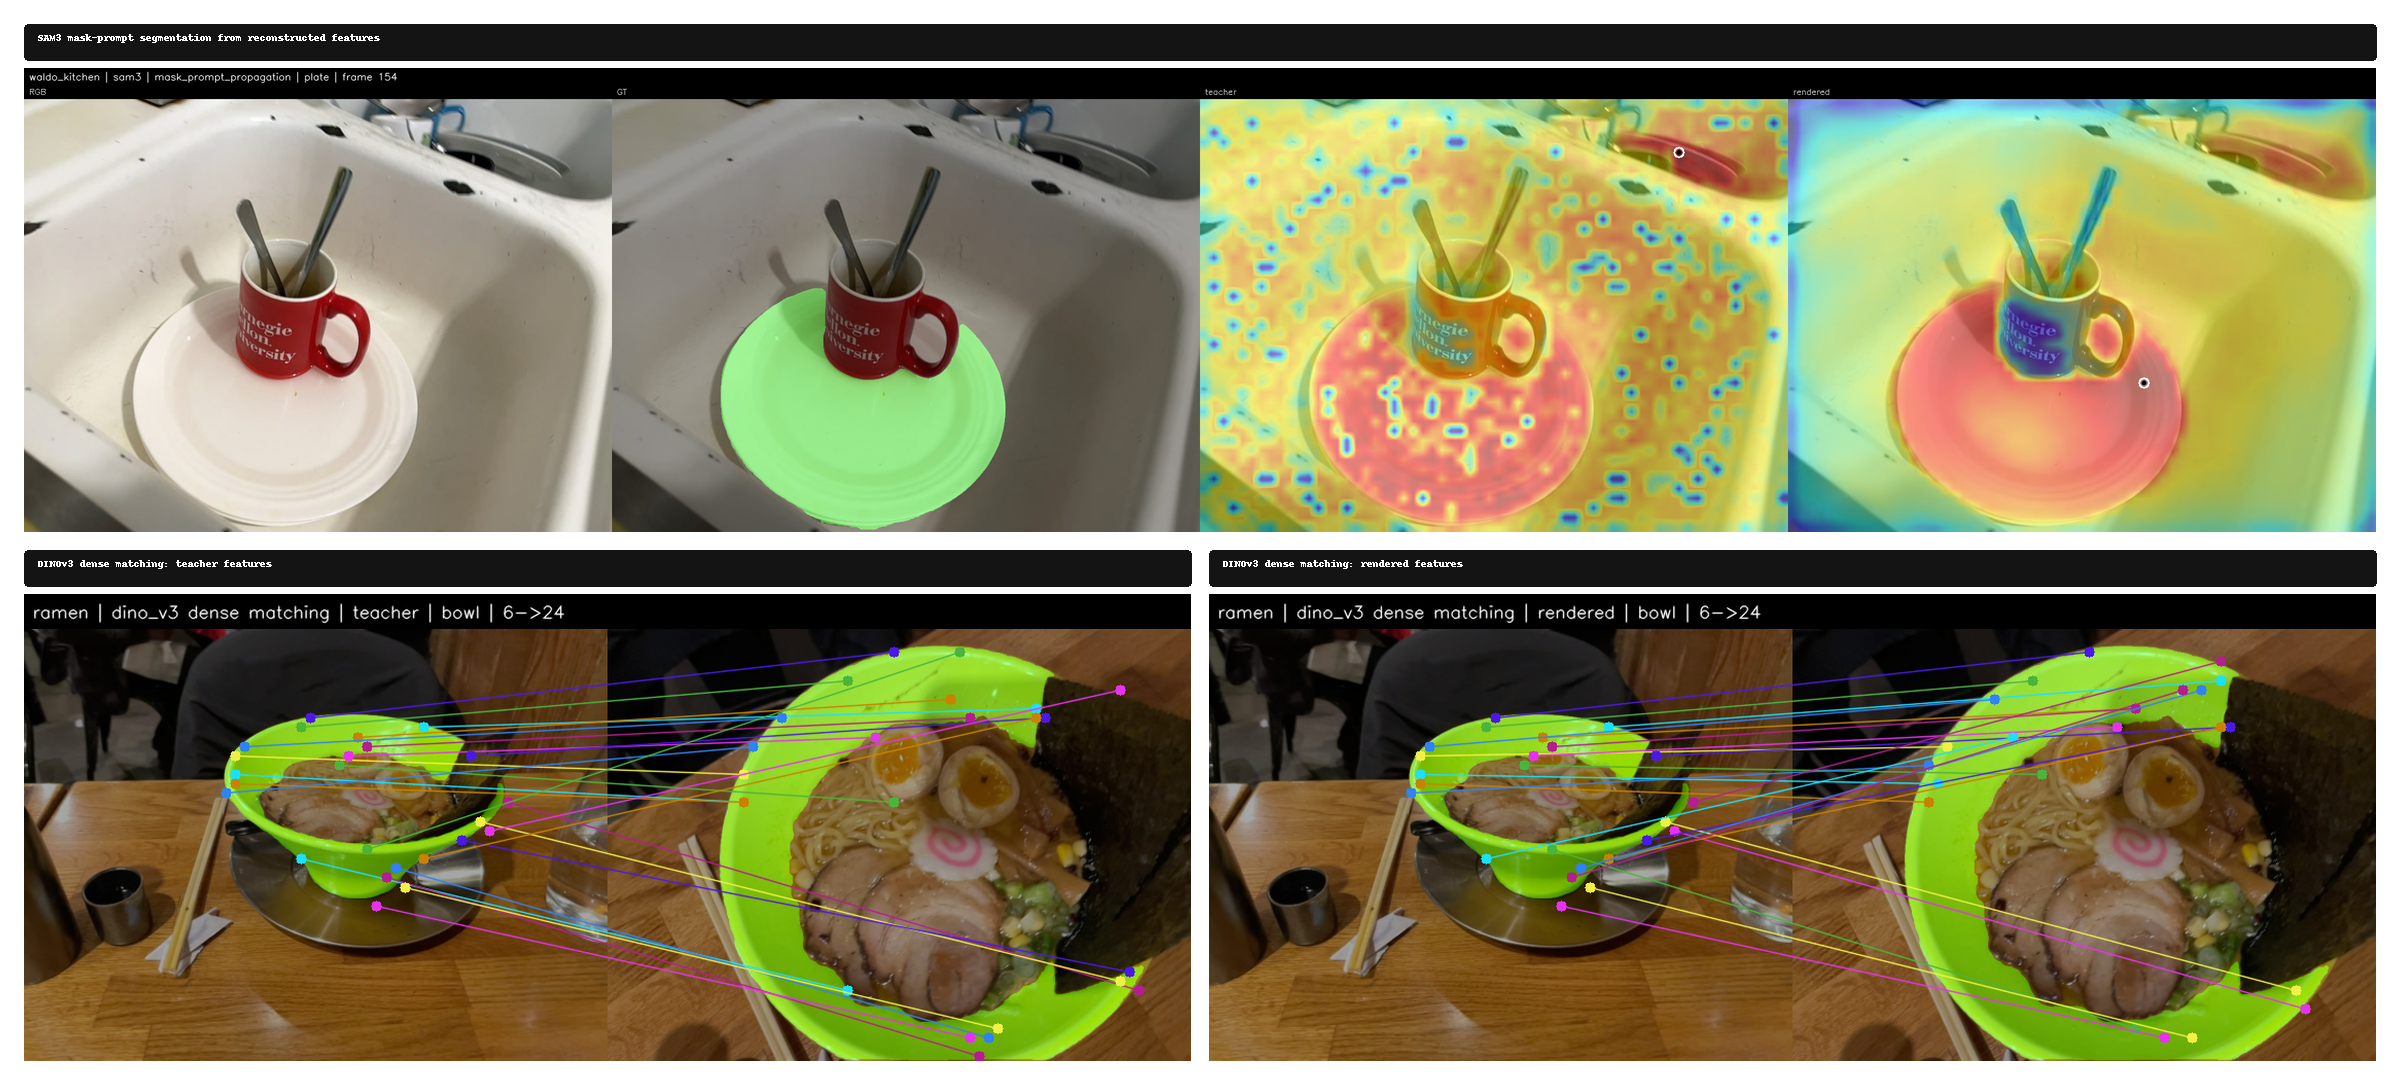
\includegraphics[width=\linewidth]{figures/lerf_sam_dino_tasks_qualitative.png}
\caption{Additional frozen-head qualitative examples. The SAM3-adaptor and
DINOv3-adaptor panels are driven by reconstructed \method{} features rather than
an official RGB SAM decoder.}
\label{fig:supp_sam_dino}
\end{figure}

Figure~\ref{fig:supp_vpr_direct3d} shows the registered multiview direct-3D
control. It is included as an analysis path because Multiview Primitive
Registration transfers registered multiview support to primitives, whereas the main compact direct selection uses the deployed
compact Gaussian-center field.

\begin{figure}[t]
\centering
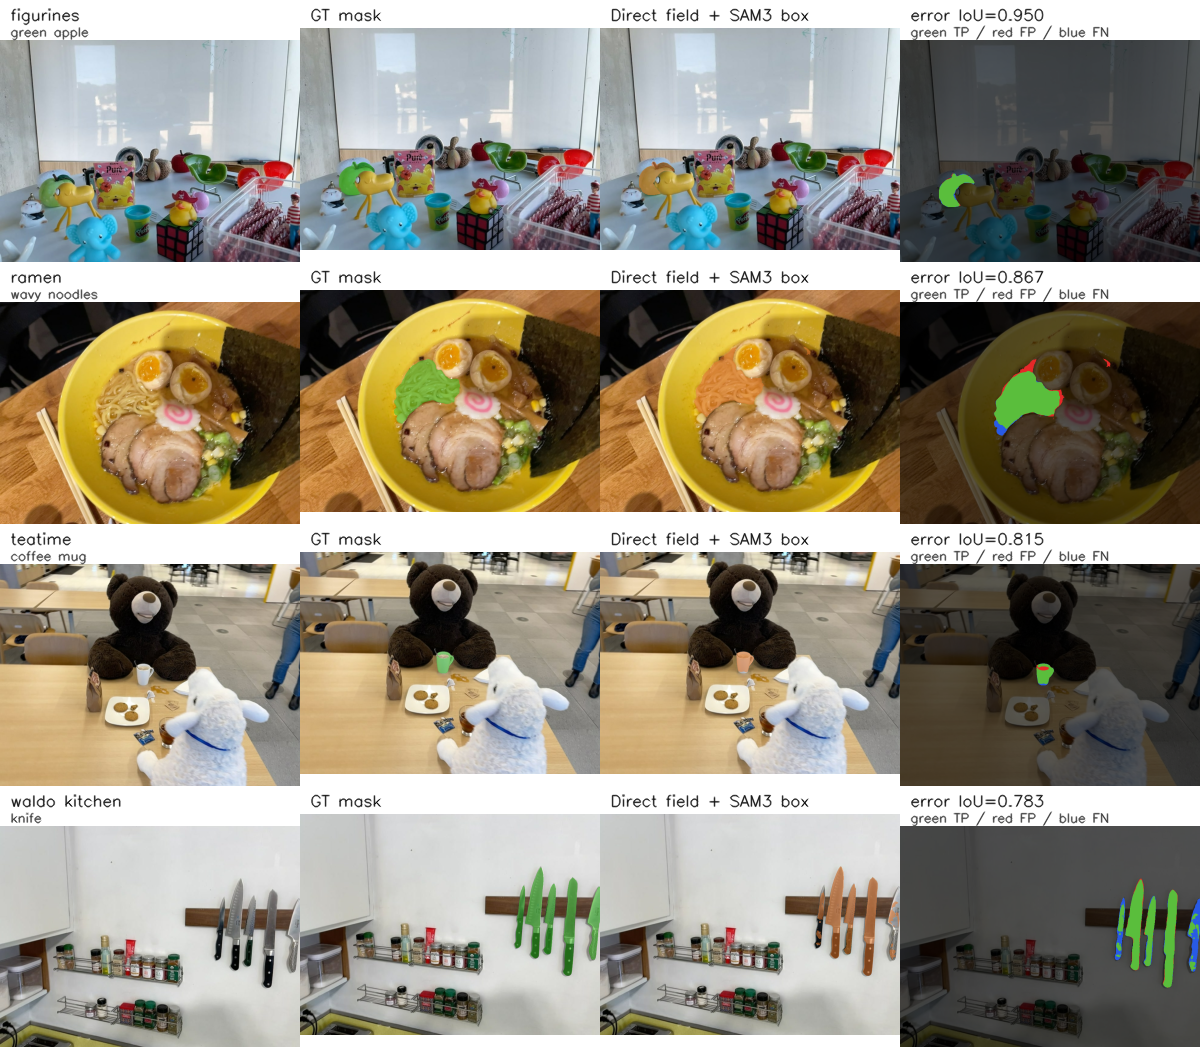
\includegraphics[width=0.86\linewidth]{figures/lerf_vpr_direct_3d_qualitative.png}
\caption{Registered multiview direct-3D control examples. Multiview Primitive
Registration is used as an analysis and training bridge, not as the main
compact-field inference cache.}
\label{fig:supp_vpr_direct3d}
\end{figure}

\begin{figure}[t]
\centering
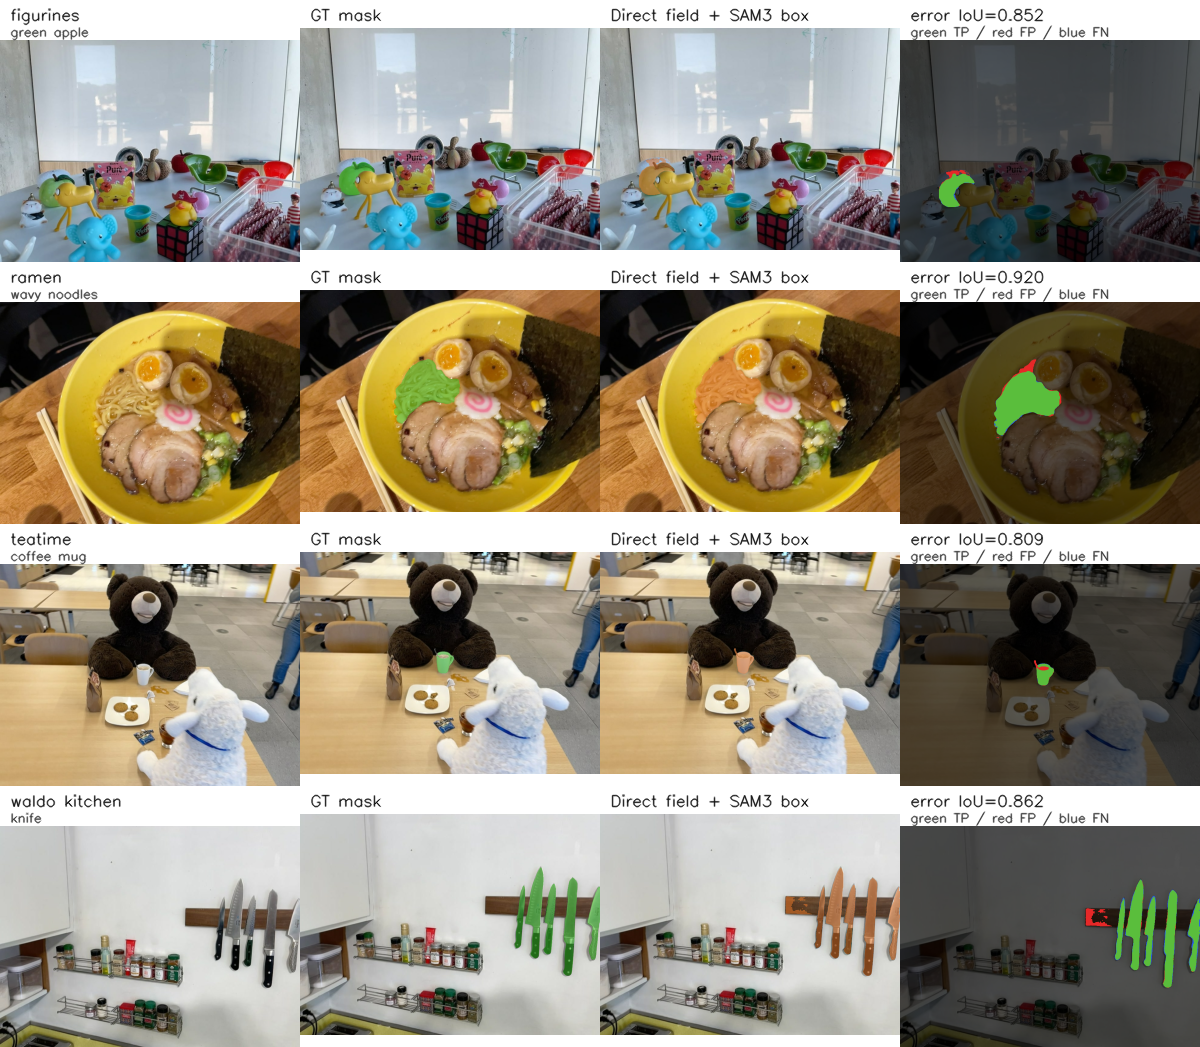
\includegraphics[width=0.86\linewidth]{figures/lerf_sam3_box_direct_3d_qualitative_pad16.png}
\caption{Boundary-assisted direct-3D examples using the SAM3-box control. This
variant illustrates a boundary diagnostic after compact primitive selection and is
separate from the strict compact one-map ablation.}
\label{fig:supp_sam3_box}
\end{figure}

\begin{figure}[t]
\centering
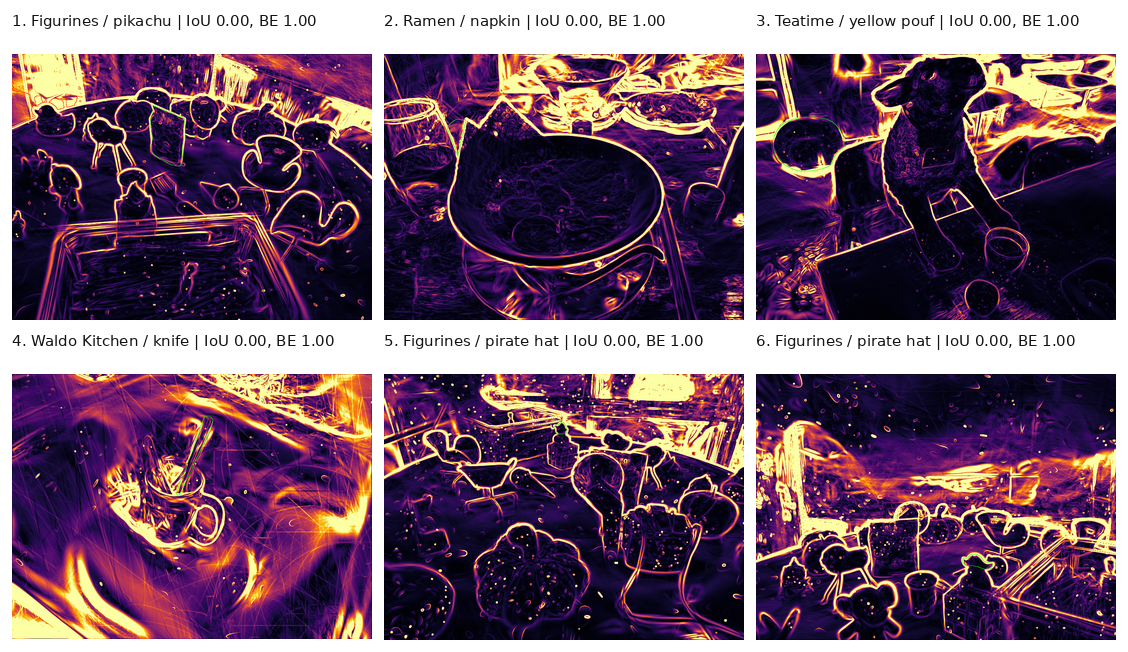
\includegraphics[width=0.92\linewidth]{figures/alpha_depth_boundary_cases.png}
\caption{Alpha/depth boundary cases used for geometric boundary analysis. These
cases expose failure modes where low object support or depth discontinuities
limit mask overlap.}
\label{fig:supp_alpha_depth}
\end{figure}

\end{document}
